\documentclass[twoside]{book}

% Packages required by doxygen
\usepackage{calc}
\usepackage{doxygen}
\usepackage{graphicx}
\usepackage[utf8]{inputenc}
\usepackage{makeidx}
\usepackage{multicol}
\usepackage{multirow}
\usepackage{textcomp}
\usepackage[table]{xcolor}

% Font selection
\usepackage[T1]{fontenc}
\usepackage{mathptmx}
\usepackage[scaled=.90]{helvet}
\usepackage{courier}
\usepackage{amssymb}
\usepackage{sectsty}
\renewcommand{\familydefault}{\sfdefault}
\allsectionsfont{%
  \fontseries{bc}\selectfont%
  \color{darkgray}%
}
\renewcommand{\DoxyLabelFont}{%
  \fontseries{bc}\selectfont%
  \color{darkgray}%
}

% Page & text layout
\usepackage{geometry}
\geometry{%
  a4paper,%
  top=2.5cm,%
  bottom=2.5cm,%
  left=2.5cm,%
  right=2.5cm%
}
\tolerance=750
\hfuzz=15pt
\hbadness=750
\setlength{\emergencystretch}{15pt}
\setlength{\parindent}{0cm}
\setlength{\parskip}{0.2cm}
\makeatletter
\renewcommand{\paragraph}{%
  \@startsection{paragraph}{4}{0ex}{-1.0ex}{1.0ex}{%
    \normalfont\normalsize\bfseries\SS@parafont%
  }%
}
\renewcommand{\subparagraph}{%
  \@startsection{subparagraph}{5}{0ex}{-1.0ex}{1.0ex}{%
    \normalfont\normalsize\bfseries\SS@subparafont%
  }%
}
\makeatother

% Headers & footers
\usepackage{fancyhdr}
\pagestyle{fancyplain}
\fancyhead[LE]{\fancyplain{}{\bfseries\thepage}}
\fancyhead[CE]{\fancyplain{}{}}
\fancyhead[RE]{\fancyplain{}{\bfseries\leftmark}}
\fancyhead[LO]{\fancyplain{}{\bfseries\rightmark}}
\fancyhead[CO]{\fancyplain{}{}}
\fancyhead[RO]{\fancyplain{}{\bfseries\thepage}}
\fancyfoot[LE]{\fancyplain{}{}}
\fancyfoot[CE]{\fancyplain{}{}}
\fancyfoot[RE]{\fancyplain{}{\bfseries\scriptsize Generated on Wed Sep 18 2013 11\-:40\-:09 for Web\-View\-Test by Doxygen }}
\fancyfoot[LO]{\fancyplain{}{\bfseries\scriptsize Generated on Wed Sep 18 2013 11\-:40\-:09 for Web\-View\-Test by Doxygen }}
\fancyfoot[CO]{\fancyplain{}{}}
\fancyfoot[RO]{\fancyplain{}{}}
\renewcommand{\footrulewidth}{0.4pt}
\renewcommand{\chaptermark}[1]{%
  \markboth{#1}{}%
}
\renewcommand{\sectionmark}[1]{%
  \markright{\thesection\ #1}%
}

% Indices & bibliography
\usepackage{natbib}
\usepackage[titles]{tocloft}
\setcounter{tocdepth}{3}
\setcounter{secnumdepth}{5}
\makeindex

% Hyperlinks (required, but should be loaded last)
\usepackage{ifpdf}
\ifpdf
  \usepackage[pdftex,pagebackref=true]{hyperref}
\else
  \usepackage[ps2pdf,pagebackref=true]{hyperref}
\fi
\hypersetup{%
  colorlinks=true,%
  linkcolor=blue,%
  citecolor=blue,%
  unicode%
}

% Custom commands
\newcommand{\clearemptydoublepage}{%
  \newpage{\pagestyle{empty}\cleardoublepage}%
}


%===== C O N T E N T S =====

\begin{document}

% Titlepage & ToC
\hypersetup{pageanchor=false}
\pagenumbering{roman}
\begin{titlepage}
\vspace*{7cm}
\begin{center}%
{\Large Web\-View\-Test \\[1ex]\large 1.\-0 }\\
\vspace*{1cm}
{\large Generated by Doxygen 1.8.5}\\
\vspace*{0.5cm}
{\small Wed Sep 18 2013 11:40:09}\\
\end{center}
\end{titlepage}
\clearemptydoublepage
\tableofcontents
\clearemptydoublepage
\pagenumbering{arabic}
\hypersetup{pageanchor=true}

%--- Begin generated contents ---
\chapter{Web\-View\-Test documentation}
\label{index}\hypertarget{index}{}\hypertarget{index_intro_sec}{}\section{Sample Project \-: Web\-View\-Test}\label{index_intro_sec}
The Web\-View\-Test project is an example of how to create 2 way communication with content loaded inside a Web\-View using Javascript

The included index.\-html file can communicate back via javascript with a host i\-O\-S or Android app. For this example only the i\-O\-S callback is relevant.\hypertarget{index_objc_to_java}{}\subsection{Objective C to Javascript}\label{index_objc_to_java}
Objective C to Javascript communication is achieved with the Web\-View method \mbox{[}webview string\-By\-Evaluating\-Java\-Script\-From\-String\-:string\mbox{]} refer to Apple's documentation for further details.

In this example we use this communications in the \hyperlink{interface_view_controller}{View\-Controller} class on the methods test\-Javascript\-:(id)sender and web\-View\-Did\-Finish\-Load\-:(\-U\-I\-Web\-View $\ast$)web\-View.

The javascript calls used for Objective C to Javascript in the html are\-:


\begin{DoxyItemize}
\item set\-Host\-App(\char`\"{}i\-O\-S\char`\"{})
\end{DoxyItemize}

Sets an internal variable (host\-App) that specifies if the host app is i\-O\-S or Android to later perform Javascript to Objective C communication\hypertarget{index_java_to_objc}{}\subsection{Javascript to Objective C}\label{index_java_to_objc}
Javascript to Objective C communication is achieved via the Web\-View\-Delegate method web\-View\-:(\-U\-I\-Web\-View $\ast$)web\-View should\-Start\-Load\-With\-Request\-:(\-N\-S\-U\-R\-L\-Request $\ast$)request navigation\-Type\-:(\-U\-I\-Web\-View\-Navigation\-Type)navigation\-Type refer to Apple's documentation for further details.

The Javascript call that communicates back to Objective C is


\begin{DoxyItemize}
\item say\-Hello()
\end{DoxyItemize}

This function will communicate with the host app. It supports communication to i\-O\-S and to Android

Once the content is loaded on the Web\-View, we make a call to set\-Host\-App(\char`\"{}i\-O\-S\char`\"{}) to specify i\-O\-S as the host app. After that, the javascript call say\-Hello() will use the internal variable host\-App to use the appropiate communication method.

For i\-O\-S it will be to attempt to launch a custom scheme 'app\-://test' that we can detect in the (U\-I\-Web\-View $\ast$)web\-View should\-Start\-Load\-With\-Request\-:(\-N\-S\-U\-R\-L\-Request $\ast$)request navigation\-Type\-:(\-U\-I\-Web\-View\-Navigation\-Type)navigation\-Type Web\-View delegate method 
\chapter{Hierarchical Index}
\section{Class Hierarchy}
This inheritance list is sorted roughly, but not completely, alphabetically\-:\begin{DoxyCompactList}
\item \contentsline{section}{Controller}{\pageref{class_controller}}{}
\item $<$U\-I\-Application\-Delegate$>$\begin{DoxyCompactList}
\item \contentsline{section}{App\-Delegate}{\pageref{interface_app_delegate}}{}
\end{DoxyCompactList}
\item U\-I\-Responder\begin{DoxyCompactList}
\item \contentsline{section}{App\-Delegate}{\pageref{interface_app_delegate}}{}
\end{DoxyCompactList}
\item U\-I\-View\-Controller\begin{DoxyCompactList}
\item \contentsline{section}{View\-Controller}{\pageref{interface_view_controller}}{}
\end{DoxyCompactList}
\item $<$U\-I\-Web\-View\-Delegate$>$\begin{DoxyCompactList}
\item \contentsline{section}{View\-Controller}{\pageref{interface_view_controller}}{}
\end{DoxyCompactList}
\end{DoxyCompactList}

\chapter{Data Structure Index}
\section{Data Structures}
Here are the data structures with brief descriptions\-:\begin{DoxyCompactList}
\item\contentsline{section}{\hyperlink{interface_app_delegate}{App\-Delegate} }{\pageref{interface_app_delegate}}{}
\item\contentsline{section}{\hyperlink{class_controller}{Controller} }{\pageref{class_controller}}{}
\item\contentsline{section}{\hyperlink{interface_view_controller}{View\-Controller} }{\pageref{interface_view_controller}}{}
\end{DoxyCompactList}

\chapter{File Index}
\section{File List}
Here is a list of all files with brief descriptions\-:\begin{DoxyCompactList}
\item\contentsline{section}{Webview\-Test/\hyperlink{_app_delegate_8h}{App\-Delegate.\-h} }{\pageref{_app_delegate_8h}}{}
\item\contentsline{section}{Webview\-Test/\hyperlink{_app_delegate_8m}{App\-Delegate.\-m} }{\pageref{_app_delegate_8m}}{}
\item\contentsline{section}{Webview\-Test/\hyperlink{main_8m}{main.\-m} }{\pageref{main_8m}}{}
\item\contentsline{section}{Webview\-Test/\hyperlink{_view_controller_8h}{View\-Controller.\-h} }{\pageref{_view_controller_8h}}{}
\item\contentsline{section}{Webview\-Test/\hyperlink{_view_controller_8m}{View\-Controller.\-m} }{\pageref{_view_controller_8m}}{}
\end{DoxyCompactList}

\chapter{Data Structure Documentation}
\hypertarget{interface_app_delegate}{\section{App\-Delegate Class Reference}
\label{interface_app_delegate}\index{App\-Delegate@{App\-Delegate}}
}


{\ttfamily \#import $<$App\-Delegate.\-h$>$}

Inheritance diagram for App\-Delegate\-:\begin{figure}[H]
\begin{center}
\leavevmode
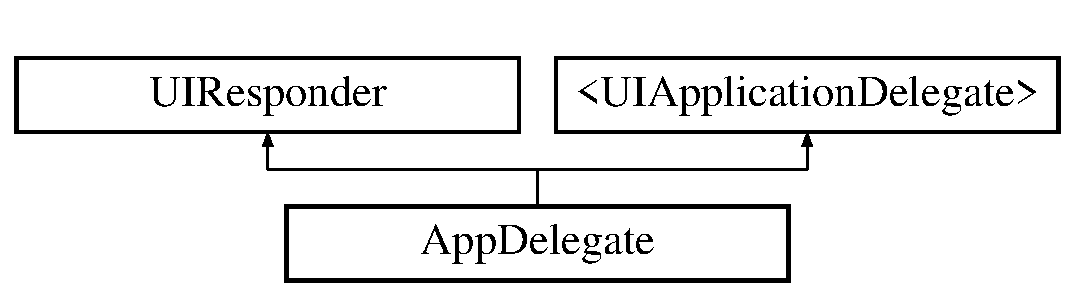
\includegraphics[height=2.000000cm]{interface_app_delegate}
\end{center}
\end{figure}
\subsection*{Instance Methods}
\begin{DoxyCompactItemize}
\item 
(B\-O\-O\-L) -\/ \hyperlink{interface_app_delegate_a0eeb7690788c7164f03af6252048d198}{application\-:did\-Finish\-Launching\-With\-Options\-:}{\ttfamily  \mbox{[}implementation\mbox{]}}
\item 
(void) -\/ \hyperlink{interface_app_delegate_ad4e9549671ce8c4fc31bd6e4836b5a91}{application\-Will\-Resign\-Active\-:}{\ttfamily  \mbox{[}implementation\mbox{]}}
\item 
(void) -\/ \hyperlink{interface_app_delegate_a26d9be79224184ef974a09c1793eb360}{application\-Did\-Enter\-Background\-:}{\ttfamily  \mbox{[}implementation\mbox{]}}
\item 
(void) -\/ \hyperlink{interface_app_delegate_ad9916739a43349edad2877110be31059}{application\-Will\-Enter\-Foreground\-:}{\ttfamily  \mbox{[}implementation\mbox{]}}
\item 
(void) -\/ \hyperlink{interface_app_delegate_a73aa814398c205f47f21ed59b616e492}{application\-Did\-Become\-Active\-:}{\ttfamily  \mbox{[}implementation\mbox{]}}
\item 
(void) -\/ \hyperlink{interface_app_delegate_ae08d55e0d58680354fceb7c8341055eb}{application\-Will\-Terminate\-:}{\ttfamily  \mbox{[}implementation\mbox{]}}
\end{DoxyCompactItemize}
\subsection*{Properties}
\begin{DoxyCompactItemize}
\item 
U\-I\-Window $\ast$ \hyperlink{interface_app_delegate_acf48ac24125e688cac1a85445cd7fac2}{window}
\item 
\hyperlink{interface_view_controller}{View\-Controller} $\ast$ \hyperlink{interface_app_delegate_afdae0acffddf96a8e7930b1151734078}{view\-Controller}
\end{DoxyCompactItemize}


\subsection{Method Documentation}
\hypertarget{interface_app_delegate_a0eeb7690788c7164f03af6252048d198}{\index{App\-Delegate@{App\-Delegate}!application\-:did\-Finish\-Launching\-With\-Options\-:@{application\-:did\-Finish\-Launching\-With\-Options\-:}}
\index{application\-:did\-Finish\-Launching\-With\-Options\-:@{application\-:did\-Finish\-Launching\-With\-Options\-:}!AppDelegate@{App\-Delegate}}
\subsubsection[{application\-:did\-Finish\-Launching\-With\-Options\-:}]{\setlength{\rightskip}{0pt plus 5cm}-\/ (B\-O\-O\-L) application\-: 
\begin{DoxyParamCaption}
\item[{(U\-I\-Application $\ast$)}]{application}
\item[{didFinishLaunchingWithOptions:(N\-S\-Dictionary $\ast$)}]{launch\-Options}
\end{DoxyParamCaption}
\hspace{0.3cm}{\ttfamily [implementation]}}}\label{interface_app_delegate_a0eeb7690788c7164f03af6252048d198}
\hypertarget{interface_app_delegate_a73aa814398c205f47f21ed59b616e492}{\index{App\-Delegate@{App\-Delegate}!application\-Did\-Become\-Active\-:@{application\-Did\-Become\-Active\-:}}
\index{application\-Did\-Become\-Active\-:@{application\-Did\-Become\-Active\-:}!AppDelegate@{App\-Delegate}}
\subsubsection[{application\-Did\-Become\-Active\-:}]{\setlength{\rightskip}{0pt plus 5cm}-\/ (void) application\-Did\-Become\-Active\-: 
\begin{DoxyParamCaption}
\item[{(U\-I\-Application $\ast$)}]{application}
\end{DoxyParamCaption}
\hspace{0.3cm}{\ttfamily [implementation]}}}\label{interface_app_delegate_a73aa814398c205f47f21ed59b616e492}
\hypertarget{interface_app_delegate_a26d9be79224184ef974a09c1793eb360}{\index{App\-Delegate@{App\-Delegate}!application\-Did\-Enter\-Background\-:@{application\-Did\-Enter\-Background\-:}}
\index{application\-Did\-Enter\-Background\-:@{application\-Did\-Enter\-Background\-:}!AppDelegate@{App\-Delegate}}
\subsubsection[{application\-Did\-Enter\-Background\-:}]{\setlength{\rightskip}{0pt plus 5cm}-\/ (void) application\-Did\-Enter\-Background\-: 
\begin{DoxyParamCaption}
\item[{(U\-I\-Application $\ast$)}]{application}
\end{DoxyParamCaption}
\hspace{0.3cm}{\ttfamily [implementation]}}}\label{interface_app_delegate_a26d9be79224184ef974a09c1793eb360}
\hypertarget{interface_app_delegate_ad9916739a43349edad2877110be31059}{\index{App\-Delegate@{App\-Delegate}!application\-Will\-Enter\-Foreground\-:@{application\-Will\-Enter\-Foreground\-:}}
\index{application\-Will\-Enter\-Foreground\-:@{application\-Will\-Enter\-Foreground\-:}!AppDelegate@{App\-Delegate}}
\subsubsection[{application\-Will\-Enter\-Foreground\-:}]{\setlength{\rightskip}{0pt plus 5cm}-\/ (void) application\-Will\-Enter\-Foreground\-: 
\begin{DoxyParamCaption}
\item[{(U\-I\-Application $\ast$)}]{application}
\end{DoxyParamCaption}
\hspace{0.3cm}{\ttfamily [implementation]}}}\label{interface_app_delegate_ad9916739a43349edad2877110be31059}
\hypertarget{interface_app_delegate_ad4e9549671ce8c4fc31bd6e4836b5a91}{\index{App\-Delegate@{App\-Delegate}!application\-Will\-Resign\-Active\-:@{application\-Will\-Resign\-Active\-:}}
\index{application\-Will\-Resign\-Active\-:@{application\-Will\-Resign\-Active\-:}!AppDelegate@{App\-Delegate}}
\subsubsection[{application\-Will\-Resign\-Active\-:}]{\setlength{\rightskip}{0pt plus 5cm}-\/ (void) application\-Will\-Resign\-Active\-: 
\begin{DoxyParamCaption}
\item[{(U\-I\-Application $\ast$)}]{application}
\end{DoxyParamCaption}
\hspace{0.3cm}{\ttfamily [implementation]}}}\label{interface_app_delegate_ad4e9549671ce8c4fc31bd6e4836b5a91}
\hypertarget{interface_app_delegate_ae08d55e0d58680354fceb7c8341055eb}{\index{App\-Delegate@{App\-Delegate}!application\-Will\-Terminate\-:@{application\-Will\-Terminate\-:}}
\index{application\-Will\-Terminate\-:@{application\-Will\-Terminate\-:}!AppDelegate@{App\-Delegate}}
\subsubsection[{application\-Will\-Terminate\-:}]{\setlength{\rightskip}{0pt plus 5cm}-\/ (void) application\-Will\-Terminate\-: 
\begin{DoxyParamCaption}
\item[{(U\-I\-Application $\ast$)}]{application}
\end{DoxyParamCaption}
\hspace{0.3cm}{\ttfamily [implementation]}}}\label{interface_app_delegate_ae08d55e0d58680354fceb7c8341055eb}


\subsection{Property Documentation}
\hypertarget{interface_app_delegate_afdae0acffddf96a8e7930b1151734078}{\index{App\-Delegate@{App\-Delegate}!view\-Controller@{view\-Controller}}
\index{view\-Controller@{view\-Controller}!AppDelegate@{App\-Delegate}}
\subsubsection[{view\-Controller}]{\setlength{\rightskip}{0pt plus 5cm}-\/ ({\bf View\-Controller}$\ast$) view\-Controller\hspace{0.3cm}{\ttfamily [read]}, {\ttfamily [write]}, {\ttfamily [nonatomic]}, {\ttfamily [strong]}}}\label{interface_app_delegate_afdae0acffddf96a8e7930b1151734078}
\hypertarget{interface_app_delegate_acf48ac24125e688cac1a85445cd7fac2}{\index{App\-Delegate@{App\-Delegate}!window@{window}}
\index{window@{window}!AppDelegate@{App\-Delegate}}
\subsubsection[{window}]{\setlength{\rightskip}{0pt plus 5cm}-\/ (U\-I\-Window$\ast$) window\hspace{0.3cm}{\ttfamily [read]}, {\ttfamily [write]}, {\ttfamily [nonatomic]}, {\ttfamily [strong]}}}\label{interface_app_delegate_acf48ac24125e688cac1a85445cd7fac2}


The documentation for this class was generated from the following files\-:\begin{DoxyCompactItemize}
\item 
Webview\-Test/\hyperlink{_app_delegate_8h}{App\-Delegate.\-h}\item 
Webview\-Test/\hyperlink{_app_delegate_8m}{App\-Delegate.\-m}\end{DoxyCompactItemize}

\hypertarget{class_controller}{\section{Controller Class Reference}
\label{class_controller}\index{Controller@{Controller}}
}


\subsection{Detailed Description}
load test content on a Web\-View and do 2 way communication via Javascript 

The documentation for this class was generated from the following file\-:\begin{DoxyCompactItemize}
\item 
Webview\-Test/\hyperlink{_view_controller_8h}{View\-Controller.\-h}\end{DoxyCompactItemize}

\hypertarget{interface_view_controller}{\section{View\-Controller Class Reference}
\label{interface_view_controller}\index{View\-Controller@{View\-Controller}}
}


{\ttfamily \#import $<$View\-Controller.\-h$>$}

Inheritance diagram for View\-Controller\-:\begin{figure}[H]
\begin{center}
\leavevmode
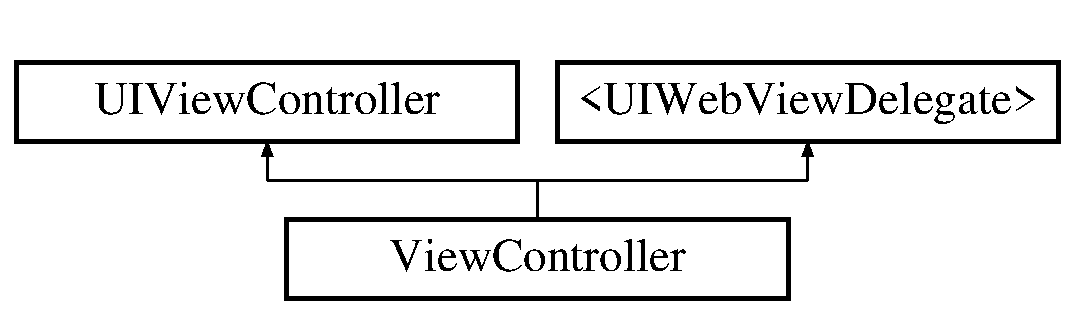
\includegraphics[height=2.000000cm]{interface_view_controller}
\end{center}
\end{figure}
\subsection*{Instance Methods}
\begin{DoxyCompactItemize}
\item 
(void) -\/ \hyperlink{interface_view_controller_aa8418c79310bb5f7235485aae32296e7}{view\-Did\-Load}{\ttfamily  \mbox{[}implementation\mbox{]}}
\begin{DoxyCompactList}\small\item\em view\-Did\-Load executed when the view has loaded \end{DoxyCompactList}\item 
(void) -\/ \hyperlink{interface_view_controller_a594064ed32a3f907d3055adb615b8662}{did\-Receive\-Memory\-Warning}{\ttfamily  \mbox{[}implementation\mbox{]}}
\begin{DoxyCompactList}\small\item\em default did\-Receive\-Memory\-Warning \end{DoxyCompactList}\item 
(void) -\/ \hyperlink{interface_view_controller_a6bf5e01d692477bccb7fd038adf226cb}{test\-Javascript\-:}{\ttfamily  \mbox{[}implementation\mbox{]}}
\begin{DoxyCompactList}\small\item\em Call triggered by the test button. \end{DoxyCompactList}\item 
(void) -\/ \hyperlink{interface_view_controller_a2de1bcd263bb715f7a8edc6c2a658a9e}{web\-View\-Did\-Finish\-Load\-:}{\ttfamily  \mbox{[}implementation\mbox{]}}
\begin{DoxyCompactList}\small\item\em Webview delegate method called when content on the Web\-View has finished loading. \end{DoxyCompactList}\item 
(B\-O\-O\-L) -\/ \hyperlink{interface_view_controller_a4176871569ddf10cd79a9fc6e5e340bb}{web\-View\-:should\-Start\-Load\-With\-Request\-:navigation\-Type\-:}{\ttfamily  \mbox{[}implementation\mbox{]}}
\begin{DoxyCompactList}\small\item\em Webview delegate method called before loading a request. \end{DoxyCompactList}\end{DoxyCompactItemize}
\subsection*{Properties}
\begin{DoxyCompactItemize}
\item 
I\-B\-Outlet U\-I\-Button $\ast$ \hyperlink{interface_view_controller_ad839c30ee296cfa982923261103473e8}{but}
\item 
I\-B\-Outlet U\-I\-Web\-View $\ast$ \hyperlink{interface_view_controller_ab7e91cb8cf4ad3747ee6a634897a9f2f}{webview}
\end{DoxyCompactItemize}


\subsection{Method Documentation}
\hypertarget{interface_view_controller_a594064ed32a3f907d3055adb615b8662}{\index{View\-Controller@{View\-Controller}!did\-Receive\-Memory\-Warning@{did\-Receive\-Memory\-Warning}}
\index{did\-Receive\-Memory\-Warning@{did\-Receive\-Memory\-Warning}!ViewController@{View\-Controller}}
\subsubsection[{did\-Receive\-Memory\-Warning}]{\setlength{\rightskip}{0pt plus 5cm}-\/ (void) did\-Receive\-Memory\-Warning 
\begin{DoxyParamCaption}
{}
\end{DoxyParamCaption}
\hspace{0.3cm}{\ttfamily [implementation]}}}\label{interface_view_controller_a594064ed32a3f907d3055adb615b8662}


default did\-Receive\-Memory\-Warning 

Nothing implemented \hypertarget{interface_view_controller_a6bf5e01d692477bccb7fd038adf226cb}{\index{View\-Controller@{View\-Controller}!test\-Javascript\-:@{test\-Javascript\-:}}
\index{test\-Javascript\-:@{test\-Javascript\-:}!ViewController@{View\-Controller}}
\subsubsection[{test\-Javascript\-:}]{\setlength{\rightskip}{0pt plus 5cm}-\/ (void) test\-Javascript\-: 
\begin{DoxyParamCaption}
\item[{(id)}]{sender}
\end{DoxyParamCaption}
\hspace{0.3cm}{\ttfamily [implementation]}}}\label{interface_view_controller_a6bf5e01d692477bccb7fd038adf226cb}


Call triggered by the test button. 

Calls the javascript function say\-Hello() inside the loaded content


\begin{DoxyParams}{Parameters}
{\em sender} & The sender of the call \\
\hline
\end{DoxyParams}
\hypertarget{interface_view_controller_aa8418c79310bb5f7235485aae32296e7}{\index{View\-Controller@{View\-Controller}!view\-Did\-Load@{view\-Did\-Load}}
\index{view\-Did\-Load@{view\-Did\-Load}!ViewController@{View\-Controller}}
\subsubsection[{view\-Did\-Load}]{\setlength{\rightskip}{0pt plus 5cm}-\/ (void) view\-Did\-Load 
\begin{DoxyParamCaption}
{}
\end{DoxyParamCaption}
\hspace{0.3cm}{\ttfamily [implementation]}}}\label{interface_view_controller_aa8418c79310bb5f7235485aae32296e7}


view\-Did\-Load executed when the view has loaded 

The webview is setup by assigning a delegate and request to load. The test button's action is setup to the selector test\-Javascript\-:


\begin{DoxyParams}{Parameters}
{\em none} & \\
\hline
\end{DoxyParams}
\begin{DoxySeeAlso}{See Also}
\hyperlink{interface_view_controller_a6bf5e01d692477bccb7fd038adf226cb}{-\/ test\-Javascript\-:}sender 

\hyperlink{interface_view_controller_a2de1bcd263bb715f7a8edc6c2a658a9e}{-\/ web\-View\-Did\-Finish\-Load\-:}web\-View 

web\-View\-:(\-U\-I\-Web\-View $\ast$)web\-View should\-Start\-Load\-With\-Request\-:(\-N\-S\-U\-R\-L\-Request $\ast$)request navigation\-Type\-:(\-U\-I\-Web\-View\-Navigation\-Type)navigation\-Type 
\end{DoxySeeAlso}
\hypertarget{interface_view_controller_a4176871569ddf10cd79a9fc6e5e340bb}{\index{View\-Controller@{View\-Controller}!web\-View\-:should\-Start\-Load\-With\-Request\-:navigation\-Type\-:@{web\-View\-:should\-Start\-Load\-With\-Request\-:navigation\-Type\-:}}
\index{web\-View\-:should\-Start\-Load\-With\-Request\-:navigation\-Type\-:@{web\-View\-:should\-Start\-Load\-With\-Request\-:navigation\-Type\-:}!ViewController@{View\-Controller}}
\subsubsection[{web\-View\-:should\-Start\-Load\-With\-Request\-:navigation\-Type\-:}]{\setlength{\rightskip}{0pt plus 5cm}-\/ (B\-O\-O\-L) web\-View\-: 
\begin{DoxyParamCaption}
\item[{(U\-I\-Web\-View $\ast$)}]{web\-View}
\item[{shouldStartLoadWithRequest:(N\-S\-U\-R\-L\-Request $\ast$)}]{request}
\item[{navigationType:(U\-I\-Web\-View\-Navigation\-Type)}]{navigation\-Type}
\end{DoxyParamCaption}
\hspace{0.3cm}{\ttfamily [implementation]}}}\label{interface_view_controller_a4176871569ddf10cd79a9fc6e5e340bb}


Webview delegate method called before loading a request. 

Used to catch an attempt to load a custom scheme 'app\-://test' to communicate from Javascript to Objective C. Launches a U\-I\-Alert\-View to confirm communication from Javascript to Objective C


\begin{DoxyParams}{Parameters}
{\em web\-View} & The Web\-View that has finished loading the request \\
\hline
{\em request} & The request being loaded \\
\hline
{\em navigation\-Type} & Constant indicating the user’s action\\
\hline
\end{DoxyParams}
\begin{DoxyReturn}{Returns}
false when the custom scheme is detected, true otherwise. 
\end{DoxyReturn}
\hypertarget{interface_view_controller_a2de1bcd263bb715f7a8edc6c2a658a9e}{\index{View\-Controller@{View\-Controller}!web\-View\-Did\-Finish\-Load\-:@{web\-View\-Did\-Finish\-Load\-:}}
\index{web\-View\-Did\-Finish\-Load\-:@{web\-View\-Did\-Finish\-Load\-:}!ViewController@{View\-Controller}}
\subsubsection[{web\-View\-Did\-Finish\-Load\-:}]{\setlength{\rightskip}{0pt plus 5cm}-\/ (void) web\-View\-Did\-Finish\-Load\-: 
\begin{DoxyParamCaption}
\item[{(U\-I\-Web\-View $\ast$)}]{web\-View}
\end{DoxyParamCaption}
\hspace{0.3cm}{\ttfamily [implementation]}}}\label{interface_view_controller_a2de1bcd263bb715f7a8edc6c2a658a9e}


Webview delegate method called when content on the Web\-View has finished loading. 

Calls the javascript function set\-Host\-App('i\-O\-S') to tell the loaded content it is loaded inside an i\-O\-S Webview


\begin{DoxyParams}{Parameters}
{\em web\-View} & The Web\-View that has finished loading the request \\
\hline
\end{DoxyParams}


\subsection{Property Documentation}
\hypertarget{interface_view_controller_ad839c30ee296cfa982923261103473e8}{\index{View\-Controller@{View\-Controller}!but@{but}}
\index{but@{but}!ViewController@{View\-Controller}}
\subsubsection[{but}]{\setlength{\rightskip}{0pt plus 5cm}-\/ (I\-B\-Outlet U\-I\-Button$\ast$) but\hspace{0.3cm}{\ttfamily [read]}, {\ttfamily [write]}, {\ttfamily [nonatomic]}, {\ttfamily [weak]}}}\label{interface_view_controller_ad839c30ee296cfa982923261103473e8}
A button to trigger a javascript test call on the content loaded in the Web\-View \hypertarget{interface_view_controller_ab7e91cb8cf4ad3747ee6a634897a9f2f}{\index{View\-Controller@{View\-Controller}!webview@{webview}}
\index{webview@{webview}!ViewController@{View\-Controller}}
\subsubsection[{webview}]{\setlength{\rightskip}{0pt plus 5cm}-\/ (I\-B\-Outlet U\-I\-Web\-View$\ast$) webview\hspace{0.3cm}{\ttfamily [read]}, {\ttfamily [write]}, {\ttfamily [nonatomic]}, {\ttfamily [weak]}}}\label{interface_view_controller_ab7e91cb8cf4ad3747ee6a634897a9f2f}
The Web\-View that will load the test content 

The documentation for this class was generated from the following files\-:\begin{DoxyCompactItemize}
\item 
Webview\-Test/\hyperlink{_view_controller_8h}{View\-Controller.\-h}\item 
Webview\-Test/\hyperlink{_view_controller_8m}{View\-Controller.\-m}\end{DoxyCompactItemize}

\chapter{File Documentation}
\hypertarget{_app_delegate_8h}{\section{Webview\-Test/\-App\-Delegate.h File Reference}
\label{_app_delegate_8h}\index{Webview\-Test/\-App\-Delegate.\-h@{Webview\-Test/\-App\-Delegate.\-h}}
}
{\ttfamily \#import $<$U\-I\-Kit/\-U\-I\-Kit.\-h$>$}\\*
\subsection*{Data Structures}
\begin{DoxyCompactItemize}
\item 
class \hyperlink{interface_app_delegate}{App\-Delegate}
\end{DoxyCompactItemize}

\hypertarget{_app_delegate_8m}{\section{Webview\-Test/\-App\-Delegate.m File Reference}
\label{_app_delegate_8m}\index{Webview\-Test/\-App\-Delegate.\-m@{Webview\-Test/\-App\-Delegate.\-m}}
}
{\ttfamily \#import \char`\"{}App\-Delegate.\-h\char`\"{}}\\*
{\ttfamily \#import \char`\"{}View\-Controller.\-h\char`\"{}}\\*

\hypertarget{main_8m}{\section{Webview\-Test/main.m File Reference}
\label{main_8m}\index{Webview\-Test/main.\-m@{Webview\-Test/main.\-m}}
}
{\ttfamily \#import $<$U\-I\-Kit/\-U\-I\-Kit.\-h$>$}\\*
{\ttfamily \#import \char`\"{}App\-Delegate.\-h\char`\"{}}\\*
\subsection*{Functions}
\begin{DoxyCompactItemize}
\item 
int \hyperlink{main_8m_a0ddf1224851353fc92bfbff6f499fa97}{main} (int argc, char $\ast$argv\mbox{[}$\,$\mbox{]})
\end{DoxyCompactItemize}


\subsection{Function Documentation}
\hypertarget{main_8m_a0ddf1224851353fc92bfbff6f499fa97}{\index{main.\-m@{main.\-m}!main@{main}}
\index{main@{main}!main.m@{main.\-m}}
\subsubsection[{main}]{\setlength{\rightskip}{0pt plus 5cm}int main (
\begin{DoxyParamCaption}
\item[{int}]{argc, }
\item[{char $\ast$}]{argv\mbox{[}$\,$\mbox{]}}
\end{DoxyParamCaption}
)}}\label{main_8m_a0ddf1224851353fc92bfbff6f499fa97}

\hypertarget{_view_controller_8h}{\section{Webview\-Test/\-View\-Controller.h File Reference}
\label{_view_controller_8h}\index{Webview\-Test/\-View\-Controller.\-h@{Webview\-Test/\-View\-Controller.\-h}}
}
{\ttfamily \#import $<$U\-I\-Kit/\-U\-I\-Kit.\-h$>$}\\*
\subsection*{Data Structures}
\begin{DoxyCompactItemize}
\item 
class \hyperlink{interface_view_controller}{View\-Controller}
\end{DoxyCompactItemize}

\hypertarget{_view_controller_8m}{\section{Webview\-Test/\-View\-Controller.m File Reference}
\label{_view_controller_8m}\index{Webview\-Test/\-View\-Controller.\-m@{Webview\-Test/\-View\-Controller.\-m}}
}
{\ttfamily \#import \char`\"{}View\-Controller.\-h\char`\"{}}\\*

%--- End generated contents ---

% Index
\newpage
\phantomsection
\addcontentsline{toc}{part}{Index}
\printindex

\end{document}
